\documentclass[conference]{IEEEtran}
\IEEEoverridecommandlockouts
% The preceding line is only needed to identify funding in the first footnote. If that is unneeded, please comment it out.
\usepackage{cite}
\usepackage{amsmath,amssymb,amsfonts}
\usepackage{algorithmic}
\usepackage{graphicx}
\usepackage{textcomp}
\usepackage{xcolor}
\usepackage{url}
\usepackage[colorlinks]{hyperref}
\usepackage{listings}
\usepackage{tikz}
\usepackage{tkz-euclide}
\usepackage{svg}

\usetikzlibrary{shapes,positioning}

\tikzset{ell/.style={circle,draw,minimum height=0.2cm,minimum width=0.2cm,inner sep=0.15cm}}


%New colors defined below
\definecolor{codegreen}{rgb}{0,0.6,0}
\definecolor{codegray}{rgb}{0.5,0.5,0.5}
\definecolor{codepurple}{rgb}{0.58,0,0.82}
\definecolor{backcolour}{rgb}{0.95,0.95,0.92}

%Code listing style named "mystyle"
\lstdefinestyle{mystyle}{
  backgroundcolor=\color{backcolour}, commentstyle=\color{codegreen},
  keywordstyle=\color{magenta},
  numberstyle=\tiny\color{codegray},
  stringstyle=\color{codepurple},
  basicstyle=\ttfamily\footnotesize,
  breakatwhitespace=false,         
  breaklines=true,                 
  captionpos=b,                    
  keepspaces=true,                 
  numbers=left,                    
  numbersep=5pt,                  
  showspaces=false,                
  showstringspaces=false,
  showtabs=false,                  
  tabsize=2
}

%"mystyle" code listing set
\lstset{style=mystyle}


\def\BibTeX{{\rm B\kern-.05em{\sc i\kern-.025em b}\kern-.08em
    T\kern-.1667em\lower.7ex\hbox{E}\kern-.125emX}}
\begin{document}

\title{Branch Prediction Models Exploration\\
\thanks{}
}
\author{\IEEEauthorblockN{Daniela Trevina}
\IEEEauthorblockA{\textit{Department of EECS} \\
\textit{Texas A\&M University-Kingsville}\\
Kingsville, USA \\
daniela.trevino@students.tamuk.edu}
\and
\IEEEauthorblockN{Daniela Lopez}
\IEEEauthorblockA{\textit{Department of EECS} \\
\textit{Texas A\&M University-Kingsville}\\
Kingsville, USA \\
daniela.lopez@students.tamuk.edu}
\and
\IEEEauthorblockN{Mengxiang Jiang}
\IEEEauthorblockA{\textit{Department of EECS} \\
\textit{Texas A\&M University-Kingsville}\\
Kingsville, USA \\
mengxiang.jiang@students.tamuk.edu}
\and
\IEEEauthorblockN{Samah Allahyani}
\IEEEauthorblockA{\textit{Department of EECS} \\
\textit{Texas A\&M University-Kingsville}\\
Kingsville, USA \\
samah.allahyani@students.tamuk.edu}
\and
\IEEEauthorblockN{Ugochukwu Onyeakazi}
\IEEEauthorblockA{\textit{Department of EECS} \\
\textit{Texas A\&M University-Kingsville}\\
Kingsville, USA \\
ugochukwu.onyeakazi@students.tamuk.edu}
}

\maketitle

\begin{abstract}
\end{abstract}

\section{Introduction}

\section{Models}
In this section, we will cover the various branch predictor models used in the simulation.
\subsection{Perceptron Predictor}
This model is a single-layer version of an artificial neural network that can identify and classify patterns, first applied to branch prediction by Jimenez and Lin\cite{jimenez2001}. In the model shown in Fig. \ref{fig:perceptron} are the input vector ($x$), the weight vector ($w$), and the output ($y$).
\begin{figure}
    \centering
    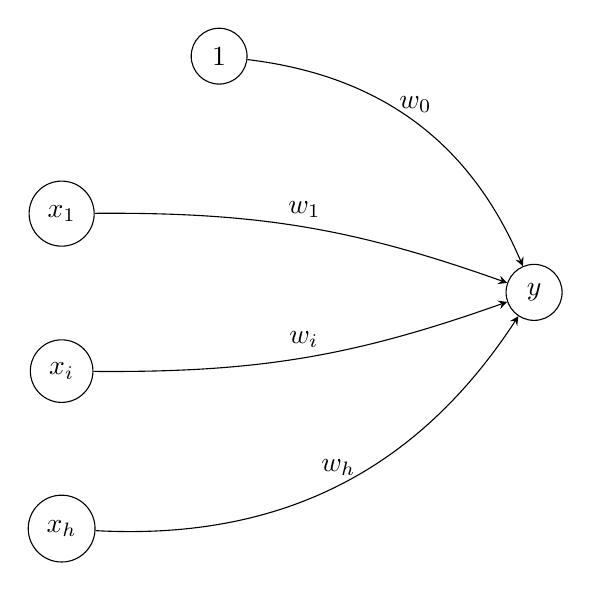
\begin{tikzpicture}[>=stealth]
		\node[ell] (x0) at (2,6) {$1$};
        \node[ell] (x1) at (0,4) {$x_1$};
        \node[ell] (xi) at (0,2) {$x_i$};
        \node[ell] (xh) at (0,0) {$x_h$};
        \node[ell] (y) at (6,3) {$y$};

        \draw [->] (x0) to [bend left]node[above]{$w_0$} (y);
		\draw [->] (x1) to [bend left=10]node[above]{$w_1$} (y);
		\draw [->] (xi) to [bend right=10]node[above]{$w_i$} (y);
		\draw [->] (xh) to [bend right]node[above]{$w_h$} (y);
    \end{tikzpicture}
    \caption{Perceptron Predictor}
	\label{fig:perceptron}
\end{figure}
The inputs correspond to values taken from the global history register, with the exception of $x_0$, the bias, always set to $1$. The output's sign determines the prediction. If it is negative, it is not taken, otherwise it is taken. Equation \eqref{eqn:1} shows the calculation of the output:
\begin{equation}
    y = w_o + \sum_{i=1}^{h}{x_iw_i}
    \label{eqn:1}
\end{equation}
The weights of the perceptron are trained using the algorithm below:
\begin{lstlisting}
if sgn(y) != t or abs(y) <= theta  then
    for i := 0 to n do
        w[i] := w[i] + t*x[i]
    end
end
\end{lstlisting}
$t$ is 1 if the branch is actually taken or -1 if not. $\theta$ is the threshold to determine when training should stop. $w_i$ is incremented if $t$ and $x_i$ agree, and decremented if they disagree.

\bibliographystyle{plain}
\bibliography{project}

\vspace{12pt}

\end{document}
